\newcommand{\Ell}{\mathcal{L}}

\subsection*{Variational inference}

Inference for the ideal point topic model requires variational updates
(see \cite{jordan:1999} for more details about variational inference).
Minimizing the KL between the variational distribution and the true
posterior is equivalent to maximizing the following lower bound on the
model evidence (called the ``evidence lower bound'', or ELBO):
\begin{align}
\log p(\bm W, \bm V) = &
\int p(\bm W, \bm V | \beta, \bm \eta, I, X, z, \theta) p(\beta, \bm \eta, I, X, z, \theta) \nonumber \\
 \geq & \expectq{\sum_D \sum_N \log p(w_n | z_n, \beta)
   + \log p(z_n | \theta_d)} \nonumber \\
& + \expectq{ \sum_D \log p(A_d, B_d | z_{d, 1:n}, \bm \eta) + \log p(\bm \eta) }\nonumber \\
& + \expectq{ \sum_U \log p(x_u) + \sum_D \log p(v_{ud} | x_u, A_d, B_d) } \nonumber \\
& + \expectq{ \sum_D \log p(\theta_d | \alpha) } + H(q) \nonumber \\
& =: \Ell(\ev, {\tilde a}, \tau, \phi, \gamma),  \label{eq:elbo}
\end{align}
where the expectations are taken with respect to the variational
distribution $q$. This bound is optimized by block coordinate ascent.
We repeatedly optimize each variational parameter until the relative
increase in the lower bound is below a specified threshold.

% dmb: we mention q here but there is no equation specifying q.  (see
% my comment above).
% smg: added it.

One important detail in this equation is that $\expectq{\log p(v_{ud}
  | x_u, A_d, B_d)}$ is not available in closed form under the variational
distribution.  We approximate the expectation in \myeq{elbo} by
applying the second-order multivariate Delta method
\cite{bickel:2007}, also applied to the logit distribution in
\cite{chang:2009,braun:2007}.  This Taylor approximation no longer
guarantees that our objective is a lower bound; however,
\cite{braun:2007} have found it to work better than a first-order
approximation (which does maintain the lower bound).

We now turn to the coordinate updates.

\paragraph{Updates for $\bm \eta$}
The variational update for $\ev$ can be found by collecting terms in
the evidence lower bound, taking the derivative with respect to $\ev$,
setting this to zero, and solving for $\ev$.  Letting $\bm
\kappa_{\mbox{disc}}$ be a bill's discrimination parameters, we
have the the exact update for the vector $\ev_{\mbox{disc}}$:
\begin{align*}
\ev_{\mbox{disc}} \gets 
 \left(\expectq{\bar{Z}^T\bar{Z}} + \frac{\sigma_d^2}{\sigma_\eta^2 } \right)^{-1}
   \expectq{\bar{Z}}^T \bm \kappa_{\mbox{disc}}. \nonumber
\end{align*}
The update for $\ev_{\mbox{diff}}$, controlling a bill's difficulty parameter $\bm \kappa_{\mbox{diff}}$, is analogous.

\paragraph{Updates for $\beta$, $\phi$, and $\gamma$}
The updates for $\beta$ and $\gamma$ are exactly as in LDA
\cite{blei:2003}, and the update for $\phi$ is exactly as in sLDA
\cite{blei:2008}; we omit details here.

\paragraph{Updates for $\kappa_d$ and $\tau_u$}
We cannot solve for $\kappa$ and $\tau$ exactly, so they must be
optimized via gradient ascent.  For bill $d$, the gradient with
respect to $\kappa$ is
\begin{align}
\label{eq:kappa_update}
\hspace{-0pt}  \nabla_{\kappa_{d,i}} \Ell(\kappa_{d, i}) =
& \sum_{D} - \frac{\kappa_{d, i} - \eta_i \overline{\phi}}{\sigma^2_d} 
 +  \sum_{v \in V(u)} 1_v {\tilde x}_{u_v, i} - {\tilde x}_{u_v, i} \rho_{ud} \nonumber \\
 & - \sum_{v \in V(d)} \frac{1}{2}
     \Big( \left( \sigma_\kappa^2 ({\tilde x}_{u_v}^T {\tilde x}_{u_v}) + \sigma_{\tilde x}^2 (\kappa_d^T \kappa_d) \right) \nonumber \\
 & \hspace{55pt} \times {\tilde x}_{u_v, i} \left( \rho_{ud} - 2 \rho_{ud}^2 + 2 \rho_{ud}^3 \right) \Big) \nonumber \\
  &  - \sum_{v \in V(d)} \frac{1}{2} \sigma_{\tilde x}^2 \Big( \kappa_{d,i} \circ
     \left( \rho_{ud}
     - \rho_{ud}^2 \right) \Big), \nonumber
\end{align}
where $\rho_{ud} = \frac{\exp(\tau_u^T \kappa_d - a_d)}{\exp(\tau_u^T
  \kappa_d - a_d) + 1}$ and $1_v$ is an indicator describing whether
vote $v$ was a \verb!yea!-vote.

To optimize this, we apply second-order gradient ascent to the sum
$\sum_d \partl{\Ell}{\kappa_d}$, repeating the updates 
\[\kappa_{d}^{n} = \kappa_{d}^{n-1} - \frac{1000}{1000 + n^{0.6}} H^{-1}\left( \nabla_{\kappa_{d}} \Ell (\kappa_{d}) \right) \]
until convergence.  In implementation, we constructed the Hessian $H$
numerically by evaluating the above gradient with coordinates
perturbed by $10^{-5}$.  For the data we used, this was sufficiently
fast; if a bill has enough votes, an alternative implementation
might use more frequent updates and fewer iterations through the
votes.

The gradient for the user-ideal parameter $\tau_u$ is nearly identical
to that for $\kappa$: 
 \begin{align}
 \label{eq:tau_update}
   \nabla{\tau_{u, i}} \Ell (\tau_{u, i}) =
 & \sum_{U} - \frac{\tau_{u, i}}{\sigma^2_u} 
  +  \sum_{v \in V(u)} 1_v \kappa_{d_v, i} - \kappa_{d_v, i} \rho_{ud} \nonumber \\
  & - \sum_{v \in V(u)} \frac{1}{2}
      \Big( \left( \sigma_\tau^2 (\kappa_{d_v}^T \kappa_{d_v}) + \sigma_\kappa^2 (\tau_u^T \tau_u) \right) \nonumber \\
  & \hspace{55pt} \times \kappa_{d_v, i} \left( \rho_{ud} - 2 \rho_{ud}^2 + 2 \rho_{ud}^3 \right) \Big) \nonumber \\
   & - \sum_{v \in V(u)} \frac{1}{2} \sigma_\kappa^2 \Big( \tau_{u,i} \circ
      \left( \rho_{ud}
      - \rho_{ud}^2 \right) \Big). \nonumber
 \end{align}
Again, we update this via second-order gradient ascent.

\paragraph{Updates for $\sigma_\kappa$ and $\sigma_{\tilde x}$.}
Once per iteration, we update the the variances $\sigma_\kappa$ and
$\sigma_{\tilde x}$.  As with $\ev$, these updates are exact:
\begin{align*}
  \sigma_\kappa^2 \gets & \frac{ND}{\sum_{D,v \in V(d)} \tau_u^T \tau_u (\rho_{u_vd} - \rho_{u_vd}^2  )_n + ND / \sigma_d^2 } \nonumber \\
  \sigma_\tau^2 \gets & \frac{NU}{\sum_{U,v \in V(u)} \kappa_d^T \kappa_d (\rho_{ud_v} - \rho_{ud_v}^2)_n + NU / \sigma_u^2 }, \nonumber \\
\end{align*}
where above we have $U$ users, $D$ bills, and an $N$-dimensional ideal-point
model.

\subsection*{B \quad Implementation details}

We provided details of a variational implementation of the ideal point
topic model.  Here we describe several modifications to improve this
algorithm.

\paragraph{Second order updates.}  Note that the second-order updates
for $\kappa$ and $\tau$ may violate the convexity assumption.  To
mitigate this, and to prevent the parameters from diverging for large
$\sigma_d$ or $\sigma_u$, we add a constant to each element of the
diagonal \cite{levenberg:1944}.  We add a sufficiently large constant
to guarantee that all $1 \times 1$ and $2 \times 2$ principal minors
have positive determinant (this is necessary but not sufficient to
guarantee that $H$ is positive definite).  We have observed that $H$
only requires this adjustment for early model iterations.

\paragraph{Identifiability.} In the modeling section, we discussed using
nonzero priors for certain legislators to make the posterior
identifiable. These priors may not be sufficient to guarantee that the
model finds specific modes.  To encourage the model to converge to the
desired optimum, we allow the first two iterations of this model one
extra dimension for the ideal point.  We believe this "blessing of
dimensionality" allows the model to rotate ideal points toward the
desired mode.

\paragraph{Annealing.}  We set the model parameters $y$ for
$\sigma_d^2$ to 1.0 before the first iteration and update it with $y
\gets y^{0.9} (\sigma_d^2)^{0.1}$ in a form of ``variational
annealing''.  We apply the same annealing to $\sigma_u$.

\section{Experimental Results.}
The experimental results for cross-fold validation are presented in
\myfig{prediction_stats}.  Top performers by various metrics are
highlighted in bold.

\begin{figure}
  \center
  \begin{tabular}{|l|l|l|l|l|}
    \hline
    \textbf{Model} & \textbf{Regularization} & \textbf{Accuracy} & \textbf{Log} & \textbf{Expected} \\
    & & & \textbf{Likelihood} & \textbf{Correct} \\
    & & & & \textbf{Probability} \\
    \hline
    \verb!lars! & 0.001 & 0.819 & \textbf{-0.855} & 0.792 \\
    \verb!lars! & 0.01 & \textbf{0.822} & -0.984 & \textbf{0.793} \\
    \verb!lars! & 0.03125 & 0.817 & -1.091 & 0.792 \\
    \verb!lars! & 0.0625 & 0.807 & -1.214 & 0.787 \\
    \verb!lars! & 0.125 & 0.799 & -1.337 & 0.781 \\
    \verb!lars! & 0.25 & 0.786 & -1.479 & 0.770 \\
    \verb!lars! & 0.5 & 0.770 & -1.640 & 0.755 \\
    \verb!lars! & 1 & 0.735 & -1.903 & 0.723 \\
    \hline
    \verb!l2! & 0.01 & 0.815 & -0.914 & 0.793 \\
    \verb!l2! & 0.1 & 0.832 & -0.794 & 0.811 \\
    \verb!l2! & 1 & 0.850 & -0.636 & 0.829 \\
    \verb!l2! & 10 & 0.876 & -0.498 & 0.853 \\
    \verb!l2! & 100 & 0.891 & -0.371 & 0.866 \\
    \verb!l2! & 1000 & \textbf{0.897} & \textbf{-0.302} & \textbf{0.868} \\
    \verb!l2! & 10000 & 0.873 & -0.324 & 0.841 \\
    \hline
    \verb!iptm! & 4 & 0.871 & -0.370 & 0.849 \\
    \verb!iptm! & 8 & 0.869 & -0.348 & 0.845 \\
    \verb!iptm! & 16 & 0.883 & -0.321 & 0.858 \\
    \verb!iptm! & 32 & 0.883 & -0.314 & 0.856 \\
    \verb!iptm! & 64 & \textbf{0.887} & \textbf{-0.306} & \textbf{0.858} \\
    \verb!iptm! & 128 & 0.873 & -0.456 & 0.845 \\
    \hline
    \verb!yea!  &     & 0.853 & -0.417 & 0.749 \\
    \hline
  \end{tabular}
  \normalsize
  \caption{Prediction metrics for heldout prediction experiments.}
  \label{fig:prediction_stats}
\end{figure}

\begin{figure}
  \center
  \begin{tabular}{|l|l|l|l|}
    \hline
    \textbf{Model} & \textbf{Accuracy} & \textbf{Log} & \textbf{Expected} \\
    & & \textbf{Likelihood} & \textbf{Correct} \\
    & & & \textbf{Probability} \\
    \hline
    \verb!l2! & 0.881 & -0.346 & 0.852 \\
    \hline
    \verb!iptm! & 0.870 & -0.346 & 0.824 \\
    \hline
    \verb!yea! & 0.851 & -0.422 & 0.746 \\
    \hline
  \end{tabular}
  \caption{Prediction metrics for time-series prediction experiments.}
  \label{fig:prediction_stats}
\end{figure}

We also display ideal points for all Senators (\myfig{senate_ideal_points}) and all legislators (Senators and House representatives) (\myfig{all_ideal_points}) in the fit of the 111th Congress.

\begin{figure}[t]
  \center
  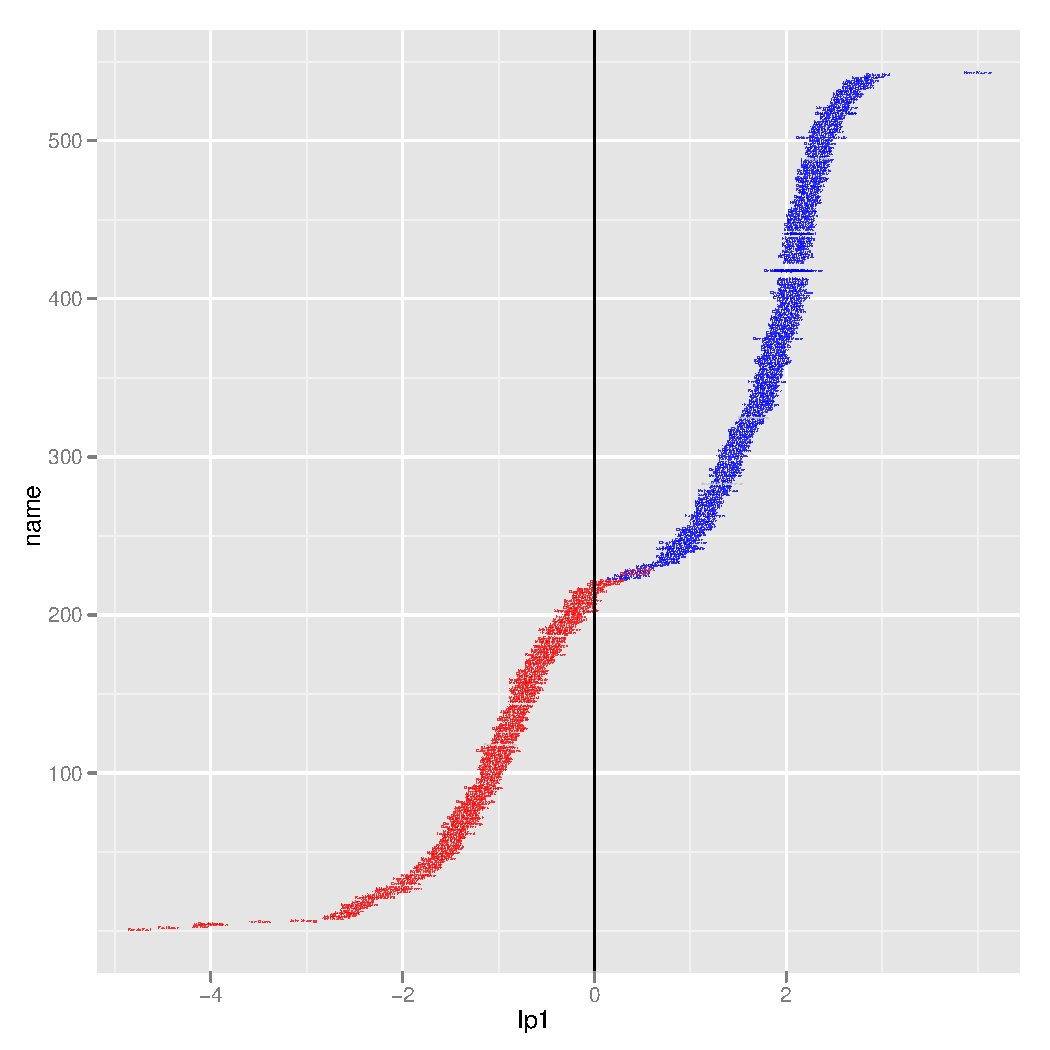
\includegraphics[width=1.\textwidth]
  {chapter_spatial_voting_with_text/figures/134_legislator_name_accuracy_by_ip.pdf}
  \caption{All legislator ideal points in the 111th Congress.  Using
    votes, ideal points can separate the U.S. political parties
    Democrats (blue) and Republicans (red).  The Y axis contains no
    information; it is used to stack names for display purposes.}
\label{fig:all_ideal_points}
\end{figure}

\begin{figure}[t]
  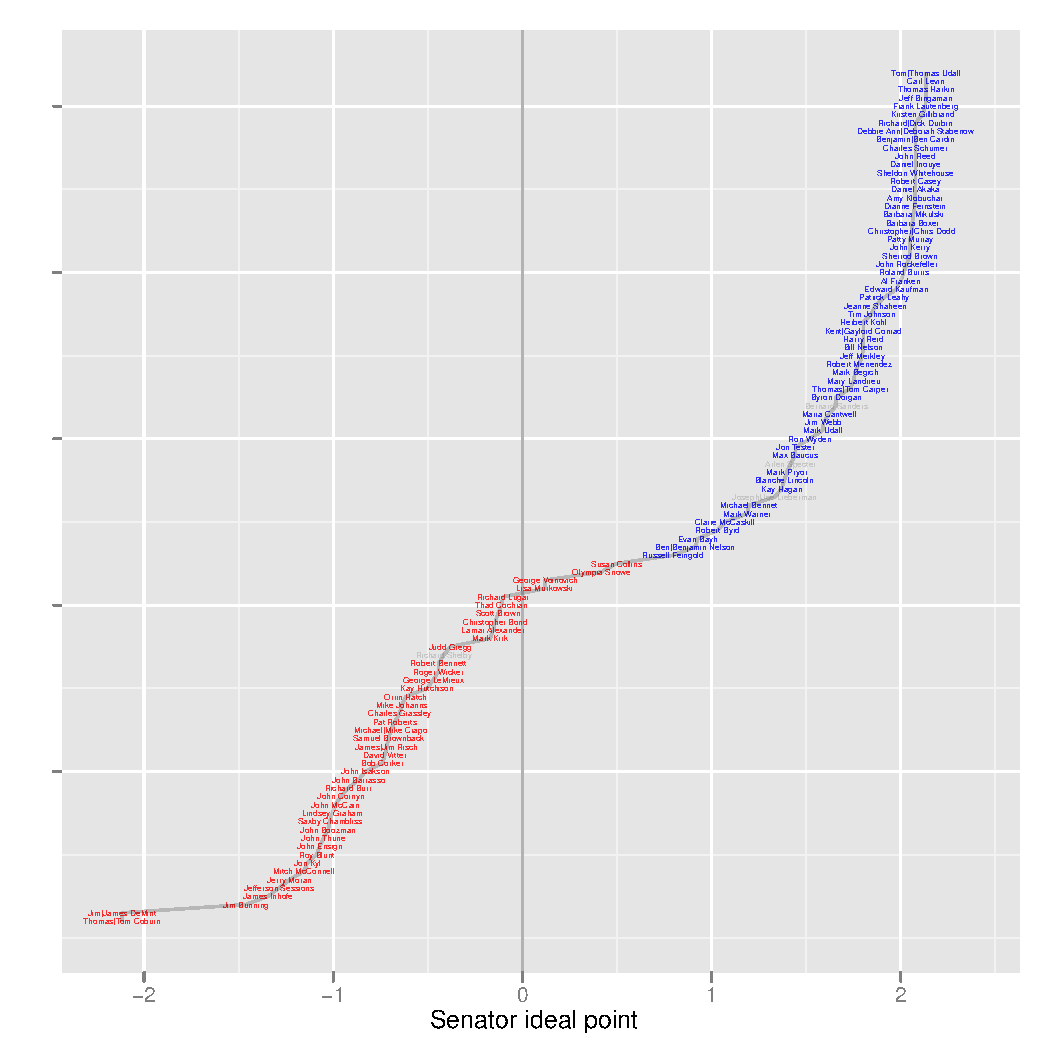
\includegraphics[width=1.\textwidth]
  {chapter_spatial_voting_with_text/figures/134_senator_name_accuracy_by_ip.pdf}
  \caption{All Senator ideal points in the 111th Congress.  Using
    votes, ideal points can separate the U.S. political parties
    Democrats (blue) and Republicans (red).}
\label{fig:senate_ideal_points}
\end{figure}


%\markright{{\bf DRAFT COPY: DO NOT CITE OR DISTRIBUTE}}
% \pagestyle{myheadings}


%% \section*{Acknowledgments}

%% \bibliographystyle{naaclhlt2010/naaclhlt2010}
%% \bibliography{../bib.bib}

%% \end{bill}
